\begin{figure}[h]
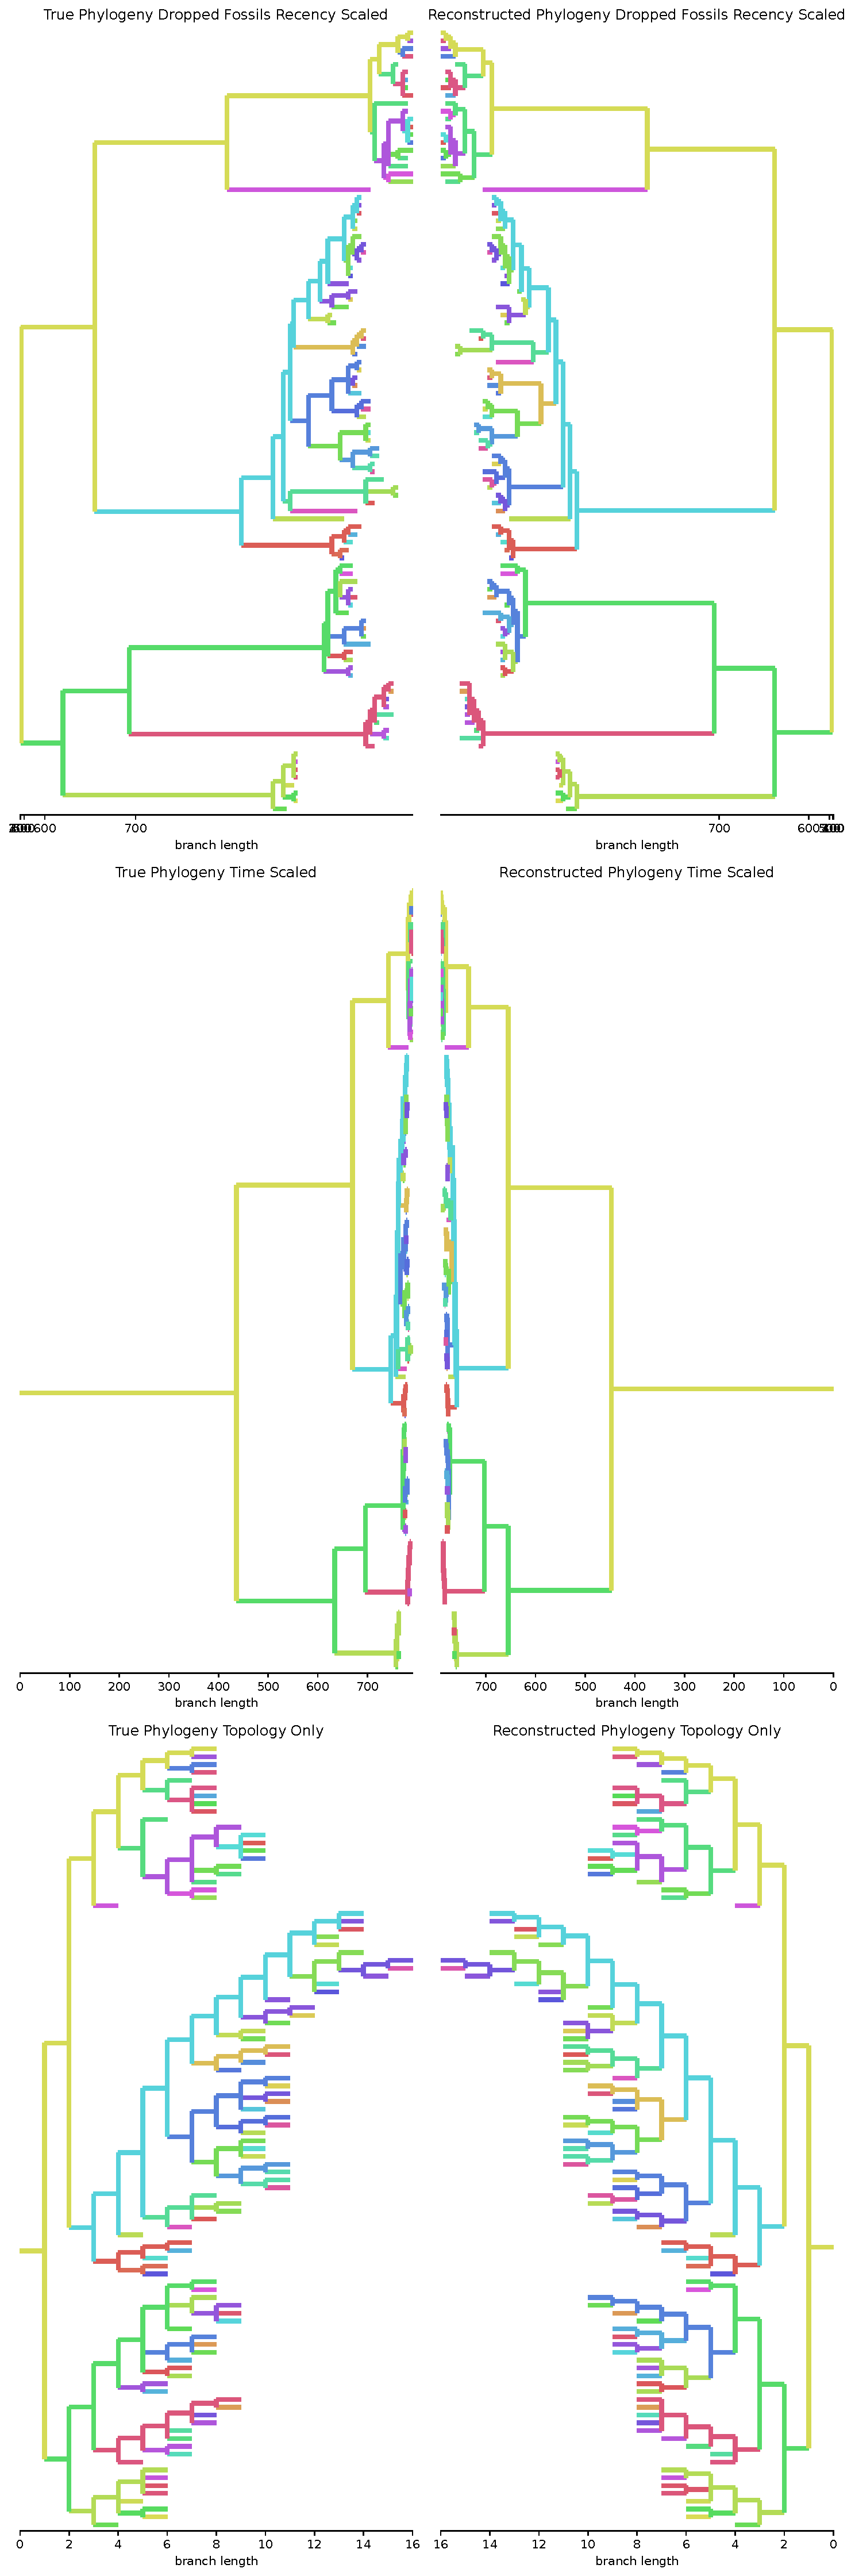
\includegraphics[width=\columnwidth,trim={0 52cm 0 0.8cm},clip]{img/colorclade.pdf}
\caption{\textbf{Sample comparison of true and reconstructed phylogenies.}
\small 
Generated using a tilted retention policy and a surface of 32 bits. The true phylogeny is on the left and the reconstructed phylogeny is on the right. Colors are based on a hash from the taxon label for each tip to better facilitate visual comparison. Reconstruction error for this reconstruction was 2.6\%. Visualization created with colorclade \citep{moreno2024colorclade}.
}
\label{fig:colorclade}
\end{figure}